\documentclass[12pt]{beamer}
\usepackage{utopia}
\usepackage{biblatex}
\bibliography{foo}
\usetheme{CambridgeUS} 
\usecolortheme{beaver}
\usepackage[utf8]{inputenc}
\usepackage{lmodern}
\usepackage{graphicx}
\graphicspath{{picture/}}
%Information to be included in the title page:
\title[DynaMIT-Database Infrastructure]
{Historical Database for DynaMIT2.0}

\author{Meng Yue}

\institute[Dep.Automation,Tsinghua]
{Department of Automation,Tsinghua University, China}

\date[August 8, 2016]
{SMART FM-IRG, August 8, 2016}
 
\logo{
\includegraphics[height=1.5cm]{combine-logo.png}}

\AtBeginSection[]
{
	\setbeamertemplate{section in toc}{{\color{red!70!black}\inserttocsectionnumber.}~\inserttocsection}
	\begin{frame}
		\frametitle{Outline}
		\tableofcontents[currentsection]
	\end{frame}
}

\setbeamertemplate{itemize items}{\color{red!70!black}$\blacktriangleright$}

\begin{document} 

\frame{\titlepage}

\begin{frame}
\setbeamertemplate{section in toc}{{\color{red!70!black}\inserttocsectionnumber.}~\inserttocsection}
\frametitle{Outline}
\tableofcontents
\end{frame}



%\section{Motivation}
%
%\begin{frame}
%\frametitle{Starting point}
%\setbeamerfont{footnote}{size=\tiny}
%The aim of the on–line calibration is to use the off–line calibrated parameter
%values as starting points and perform a local optimization step towards the unobserved true values\footnote{ Constantinos, A. (2004) On–line Calibration for Dynamic Traffic Assignment}.\\ 
%\vspace{0.5in}
%Precise historical OD-flow $=>$ Accurate estimated OD-flow \\
%
%\end{frame}
%
%\begin{frame}
%\frametitle{OD-Flow Analysis(1)}
%Altered by many factors:
%\begin{itemize}
%\item rush hour
%\item weather
%\item holiday
%\item ...
%\end{itemize}
%%TODO Maybe needs a comparison of od-flow between morning an noon.
%\vspace{0.5in}
%Needs to be stratified under several tags
%\end{frame}
%
%\begin{frame}
%\frametitle{OD-flow analysis(2)}
%\begin{itemize}
%\item The historical data may be not accurate at first.\\
%\vspace{0.5in}
%\item Needs update process
%\end{itemize}
%\end{frame}
%
%
%\begin{frame}
%\frametitle{Insights}
%\setbeamerfont{footnote}{size=\tiny}
%\begin{itemize}
%\item Set up database for storage
%\item Update historical data with estimated data
%\item Provide best-fit historical flow
%\end{itemize}
%\end{frame}
%
%\begin{frame}
%\frametitle{Goal}
%To design a program that can automatically \textbf{save} results from the DynaMIT simulation ,\textbf{update} the historical OD-flow and \textbf{render} proper demand input for the real-time DynaMIT simulation.
%\end{frame}
%%TODO Here needs discussion with HaiZheng.
%

\section{DynaMIT2.0 Database}

\begin{frame}
\frametitle{Overview}
\begin{itemize}
\item Archive inputs and outputs for each day
\item Save selected inputs and output files from each run to database
\item Update historical database each day 
\item Auto-check and backup
\item Online Calibration
\end{itemize}
\end{frame}

\begin{frame}
\frametitle{Database Structure}
\vspace{-1 cm}
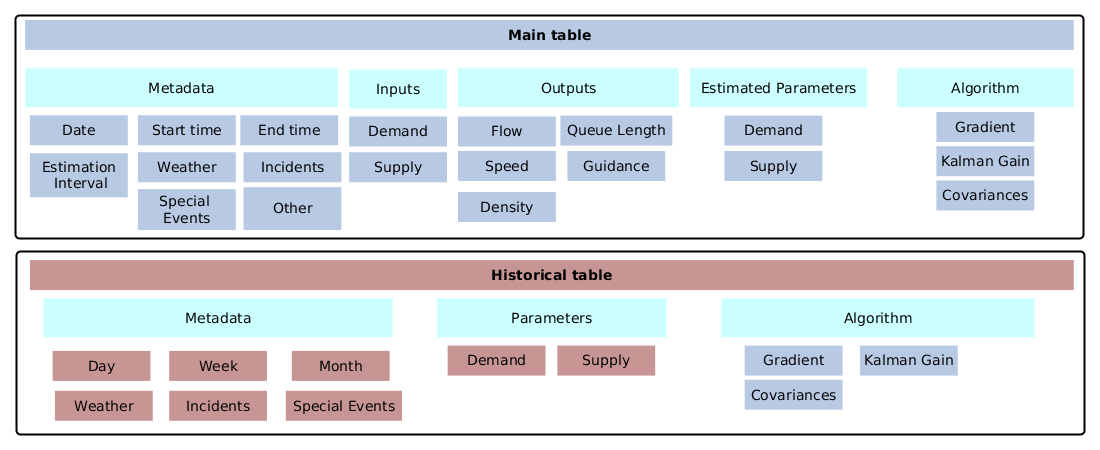
\includegraphics[scale=0.3]{table3.png}
\end{frame}





\begin{frame}
\frametitle{Testing}

\begin{center}
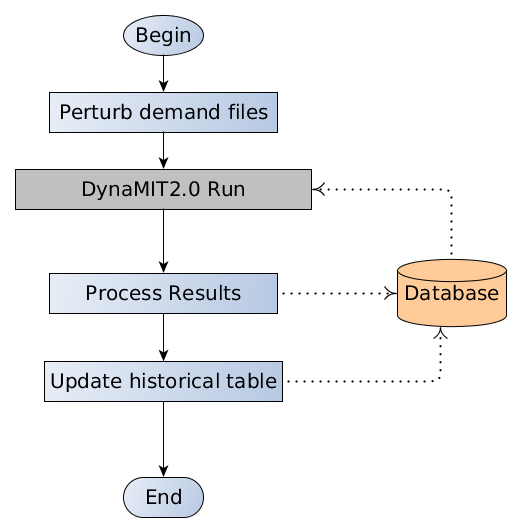
\includegraphics[scale=0.35]{flow_chart2.png}
\end{center}
\end{frame}

\begin{frame}
\frametitle{Implementation}
\begin{itemize}
\item Database: PostgreSQL
\item Language: 
\begin{itemize}
      \item{Python (file operation)}
      \item{Java (database I/D/U/Q)}
      \item{Shell (whole process)}
\end{itemize}
\end{itemize}
\end{frame}



\begin{frame}
\frametitle{Setup process}
\begin{itemize}
\item CREATE TABLE: database.config
\item Framework parameter: params.config \& init.sh
%\item Generate demands: demand\_perturb.py 
\end{itemize}
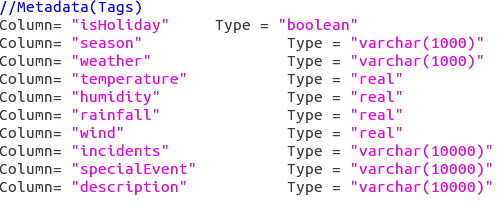
\includegraphics[width = 0.5\textwidth]{screenshot_table.png}
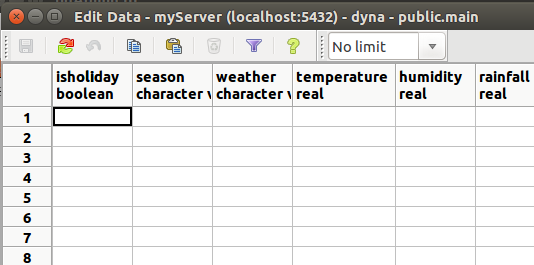
\includegraphics[width = 0.5\textwidth]{screenshot_pgadmin.png}
\end{frame}



\begin{frame}
\frametitle{Insert process(main table)}
\begin{itemize}
\item dtaparam.dat
\item behavior.dat
\item supplyparam.dat
\item sensor.out
\item demand.dat
\item estimatedOD*
\item EOD.txt
\item sen\_flw\_*
\item sen\_spd\_*
\item ...
\end{itemize}
\end{frame}

\begin{frame}
\frametitle{Update process(historical table)}
%main::estimatedOD $=>$ hod::historicalOD
%\vspace{0.3in}

%Update algorithm:
%\begin{itemize}
%\item Last EstimatedOD
%\item Moving Average
%\item Smoothing Model
%\item ...
%\end{itemize}
%\item \textbf{Algorithms for 'update process':}
\begin{itemize}
%\item Fixed historical OD-flow
\item Last estimated OD-flow
\item Simple moving average
\item Exponential moving average
\item Smoothing Model
\end{itemize}
\end{frame}

%\begin{frame}
%\frametitle{Generate historical data process}
%SELECT estimatedOD FROM hod WHERE ...  
%\end{frame}

\begin{frame}
\frametitle{Screen-shot}
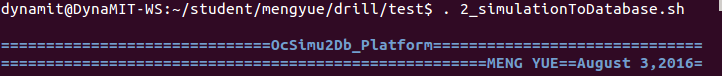
\includegraphics[width = 0.8\textwidth]{scst_1.png}
\vspace{0.1in}

\includegraphics[width = 0.8\textwidth]{scst_2.png}
\vspace{0.1in}
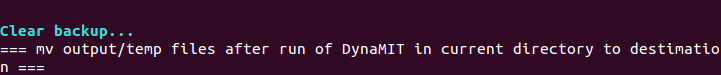
\includegraphics[width = 0.8\textwidth]{scst_3.png}
\vspace{0.1in}
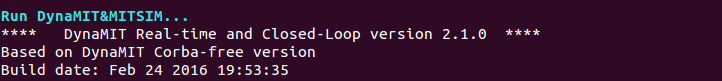
\includegraphics[width = 0.8\textwidth]{scst_4.png}
\end{frame}

\begin{frame}
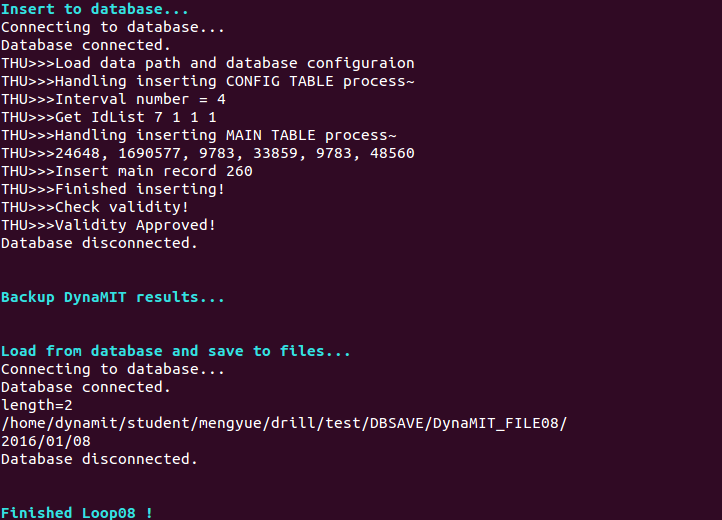
\includegraphics[width=0.8\textwidth]
{scst_5.png}
\vspace{0.1in}
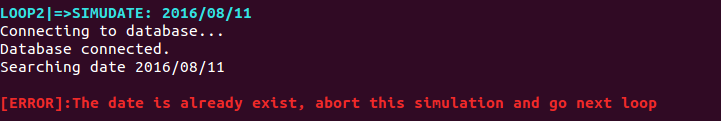
\includegraphics[width = 0.8\textwidth]{scst_6.png}
\end{frame}
\section{Experiment}

%\begin{frame}
%\frametitle{Purpose}
%\begin{itemize}
%\item Examine the historical database for DynaMIT
%\vspace{0.3in}
%\item Compare different algorithms for update process
%\end{itemize}
%\end{frame}
%
%
%\begin{frame}
%\frametitle{Design}
%\begin{itemize}
%\item Mode: DynaMIT+MITSIM,\, with on-line calibration
%\item Parameters: \,15:00-21:00,\,10 days,\,1633 OD-pairs,\, 650 sensor flow counts
%\item \textbf{Algorithms for 'update process':}
%\begin{itemize}
%\item Fixed historical OD-flow
%\item Last estimated OD-flow
%\item Simple moving average
%\item Exponential moving average
%\item Smoothing Model
%\end{itemize}
%\item Performance analysis: RMSN for sensor data
%\end{itemize}
%\end{frame}

\begin{frame}
\frametitle{Update algorithm(1)}
Fixed historical OD-flow (base):\\

\[ x_h^{H,n}=x_h^{H,n-1}=Const \]

Last estimated OD-flow:\\
\[ x_h^{H,n}=\hat{x}_h^n\]

Notation:
\begin{itemize}
\item $x_h^{H,n} \sim$ Historical OD-flow at interval $h$ after $n$ days
\item $\hat{x}_h^{n} \sim$ Estimated OD-flow at interval $h$ on the $n^{th}$ day
\end{itemize}
\end{frame}

\begin{frame}
\frametitle{Update algorithm(2):Moving Average}

Simple moving average:\\
\[ x_h^{H,n}=\frac{1}{M}(\sum_{k=0}^{M-1} \hat{x}_h^{n-k})\]
Exponential moving average:\\
\[ x_h^{H,n}=\alpha\cdot \hat{x}_h^n+ (1-\alpha) x_h^{H,n-1}\]


Notation:
\begin{itemize}
\item $x_h^{H,n} \sim$ Historical OD-flow at interval $h$ after $n$ days
\item $\hat{x}_h^{n} \sim$ Estimated OD-flow at interval $h$ on the $n^{th}$ day
\item $M\sim$ Window size
\item $\alpha\sim$ Degree of weighting decrease between zero and one
\end{itemize}
\end{frame}

\begin{frame}
\setbeamerfont{footnote}{size=\tiny}
\frametitle{Update algorithm(3):Smoothing Model\footnote{Kalidas, A. (1996) Estimation and Prediction of Time-Dependent Origin-Destination Flows}}
Smoothing model formula:\\
\[ x_h^{H,n}=x_h^{H,n-1}+\alpha(\hat{x}_h^n-x_h^{H,n-1}) \]

Notation:\\
\begin{itemize}
\item $x_h^{H,n} \sim$ Historical OD-flow at interval h after n days
\item $\hat{x}_h^{n} \sim$ Estimated OD-flow at interval h on the $n^{th}$ day 
\item $\alpha \sim$ A scalar between zero and one
\end{itemize}



\end{frame}


%\begin{frame}
%\frametitle{Measurement}
%Root Mean Square Normalized(RMSN):
%\[ RMSN=\frac{\sqrt{N\sum_{i=1}^{N} (y_i-y_i^*)^2}}{\sum_{i=1}^{N}y_i^*} \]
%
%\begin{itemize}
%\item $y_i\sim$ The $i^{th}$ sensor data calculated from DynaMIT
%\item $y_i^*\sim$ The $i^{th}$ sensor data generated from MITSIM/hist\_flow 
%\end{itemize}
%\end{frame}
%
%\begin{frame}
%\frametitle{Data excel}
%\begin{itemize}
%\item FHOD-Fixed Historical OD-flow
%\item LEOD-Last Estimated OD-flow
%\item SMA -Simple Moving Average
%\item EMA -Exponential Moving Average
%\item SM  -Smoothing Model 
%\end{itemize}
%
%\begin{table}
%\begin{center}
%\scalebox{0.7}{
%\begin{tabular}{|c|c|c|c|c|c|}
%\hline
% & FHOD & LEOD & SMA & EMA & SM\\ \hline
%Day01 &  &  &  &  &\\ \hline
%Day02 &  &  &  &  &\\ \hline
%Day03 &  &  &  &  &\\ \hline
%Day04 &  &  &  &  &\\ \hline
%Day05 &  &  &  &  &\\ \hline
%Day06 &  &  &  &  &\\ \hline
%Day07 &  &  &  &  &\\ \hline
%Day08 &  &  &  &  &\\ \hline
%Day09 &  &  &  &  &\\ \hline
%Day10 &  &  &  &  &\\ \hline
%\end{tabular}}
%\end{center}
%\end{table}
%\end{frame}
%
%\begin{frame}
%\frametitle{Anticipation}
%\begin{itemize}
%\item Update process reduces the error
%\item Error descends with iteration
%\item Algorithm with slow change may perform better than drastic one
%\end{itemize}
%\end{frame}


%\section{Summary}
%\begin{frame}
%\frametitle{Finished progress}
%\begin{itemize}
%\item Implemented a database-based simulation infrastructure 
%\begin{itemize}
%\item Define table
%\item Grab and insert data
%\item Top-level script
%\end{itemize}
%\item Designed 'update process' test
%\end{itemize}
%\end{frame}
%
%\begin{frame}
%\frametitle{Future research}
%\begin{itemize}
%\item The experiment given above
%\item Find source for the metadata
%\item Refactoring \& Documentation
%\end{itemize}
%\end{frame}

%\begin{frame}
%\frametitle{Acknowledgement}
%\setlength\parindent{24pt}
%\indent \it{Thanks Haizheng, Ravi, Samarth and Arun for offering me loads of help during the research period. Hope we still have chance to cooperate in the near future!}
%\end{frame}

\begin{frame}
\frametitle{Questions}
\begin{center}

\includegraphics[width = 0.3\textwidth]{question.png}
\end{center}
\end{frame}
 
 
\begin{frame}
\frametitle{Thank you!}
\end{frame}
\end{document}

